% CS4.406 Assignment 3 report. At most 5 pages including figures and tables.
%
% - Every number comes from a table under report/tables/ or a row of results/results.csv (the full run of
%   27 October 2026); ratios and per-distance costs are arithmetic on those values.
% - Compile locally from report/ (latexmk -pdf report.tex, or LaTeX Workshop); the figures are found in
%   ../results/figures/. Or upload the Overleaf bundle described in README.md (pdfLaTeX).
\documentclass[10pt,a4paper]{article}
\usepackage[a4paper,margin=1.8cm]{geometry}
\usepackage[T1]{fontenc}
\usepackage{lmodern,microtype,graphicx,array,booktabs,adjustbox,xcolor,newunicodechar,amsmath}
\usepackage[font=small,labelfont=bf,skip=4pt]{caption}
\usepackage[hidelinks]{hyperref}
\newunicodechar{σ}{\ensuremath{\sigma}}
\graphicspath{{figures/}{../results/figures/}}
\newcommand{\todo}[1]{\textcolor{red}{[TODO: #1]}}
\newcommand{\tableinput}[1]{\begin{adjustbox}{max width=\linewidth}\small\setlength{\tabcolsep}{4.5pt}\input{tables/#1}\end{adjustbox}}
\setlength{\parskip}{3pt}
\setlength{\parindent}{0pt}

\title{\vspace{-1.5em}Benchmarking Approximate Nearest Neighbour Search\vspace{-0.5em}}
\author{Iman Kalyan Chakraborty - 2026801003 \\ CS4.406 Information Retrieval \& Extraction, Assignment 3 \\ \small Code: \url{https://github.com/astrion-coder/ire-assignment-3}}
\date{\vspace{-1.5em}}

\begin{document}
\maketitle

% =====================================================================================================================
\section{Setup}
This assignment benchmarks three approximate nearest neighbour, or ANN, index types, HNSW, IVF-Flat and IVF-PQ, against exact
search. The comparison uses SIFT (1,000,000 vectors, 128 dimensions) and GloVe-100 (1,183,514 vectors, 100 dimensions). The benchmark normalises the GloVe vectors and uses Euclidean distance for everything. All indexes come from FAISS, while the recall function, the timing code and the plots are this project's own code. Table~\ref{tab:machine} lists the machine and the package versions used.
\begin{table}[h]\centering
\tableinput{machine}
\caption{Machine and library versions, as recorded in every row of results.csv.\label{tab:machine}}
\end{table}

Speeds are in queries per second, or QPS. The benchmark times every search one query at a time, on a single thread pinned to one performance core. Each setting gets 200 untimed warm-up queries and 3 timed passes, and the reported speed is the median pass. The benchmark times each build once, on 12 threads. It chooses every setting on queries 0--4,999 and reports every number on queries 5,000--9,999. The recall@10
function recomputes distances in float64 and counts a returned vector as correct if it is no farther than the true 10th neighbour,
with a relative tolerance of $10^{-6}$. Ties at rank 10 therefore do not count as mistakes, and the unit tests include such a tie.
The ground truth is this project's own exact search, rerun for every subset and every noise level, rather than the stored neighbours. The timings were steady. The median spread between the 3 passes of a setting was 0.3\%, and two timings of exact
search on SIFT, about an hour apart, agreed to within 1.0\%.

% =====================================================================================================================
\section{Part 1: Exact baseline}
The exact search is FAISS's \texttt{IndexFlatL2}, which compares each query with every base vector. Its results agree with the
neighbours stored in the data files. Recall@10 is 1.000 in both directions on all 10,000 queries of both datasets. The top-10 sets
are identical for 99.4\% of SIFT queries and 100\% of GloVe queries, and the remaining SIFT queries differ only by vectors tied at
rank 10.

As the assignment suggests, batching makes a large difference. On SIFT, exact search gives 47.8 QPS one query at a time, 156 QPS as one batch on a single thread (3.3$\times$) and 773 QPS on 12 threads (16.2$\times$). One query at a time, FAISS streams the entire
base matrix (512\,MB for SIFT) from RAM again for each query, which makes the search memory-bound. Each vector it loads takes part in one distance and then leaves the cache. With a batch, FAISS switches to a BLAS matrix multiplication, so a block of base vectors loaded
into the cache serves thousands of queries. This removes the memory-bandwidth bottleneck and makes the search compute-bound. Threads
can then share the computation, although 12 threads add only a further 5.0$\times$ (773 vs 156 QPS), not 12$\times$. GloVe behaves
the same way (3.1$\times$ and 14.3$\times$).

\begin{table}[h]\centering
\tableinput{part1_agreement}\\[4pt]
\tableinput{part1_timing}
\caption{Exact search. The top table compares the exact top-10 with the stored neighbours. The bottom table gives the timings, with each speed-up relative to one query at a time on the same dataset.}
\end{table}

% =====================================================================================================================
\section{Part 2: HNSW, IVF-Flat and IVF-PQ}
HNSW used $M = 8$, 16 and 32 with efConstruction 200. IVF-Flat used nlist = 1024 and 4096. IVF-PQ used nlist = 4096 with $m = 16$, 32 and 64 one-byte sub-vectors on SIFT, or 20 and 50 on GloVe. For each build the benchmark swept the
search parameter, efSearch up to 2048 or nprobe up to a quarter of the lists, until the recall on the tuning queries reached 0.995
or the grid ended. Figure~\ref{fig:part2} shows the best trade-off curve of each index. Wherever both have points, HNSW lies above
IVF-Flat on both datasets, and both lie above exact search everywhere. At recall 0.95, HNSW answers 10,951 QPS on SIFT and 1,198 on GloVe, against 2,993 and 552 for IVF-Flat and about 50 for exact search (Table~\ref{tab:part2}).

IVF-PQ never reaches 0.95, or even 0.90. Its best recall is 0.887 on SIFT ($m = 64$) and 0.868 on GloVe ($m = 50$). The cause is
quantisation. PQ stores each vector as $m$ one-byte codes, one per sub-vector, so the distances it computes are approximations.
Their error can be larger than the small gap between a query's 10th and 11th nearest neighbours, so IVF-PQ ranks neighbours wrongly
even when they are in the probed lists. Probing more lists cannot fix this, and on SIFT the $m = 64$ build gains nothing from
nprobe 384 to 1024. Longer codes raise the ceiling (0.596, 0.746 and 0.887 for $m = 16$, 32, 64). Re-ranking the top candidates
with exact distances would remove it, but this study did not use re-ranking. HNSW with $M = 8$ on GloVe also falls short and reaches only 0.897, even with efSearch 2048. With only 8 links per node the graph is too sparse for this harder data, and a wider search adds little recall.

\begin{figure}[h]\centering
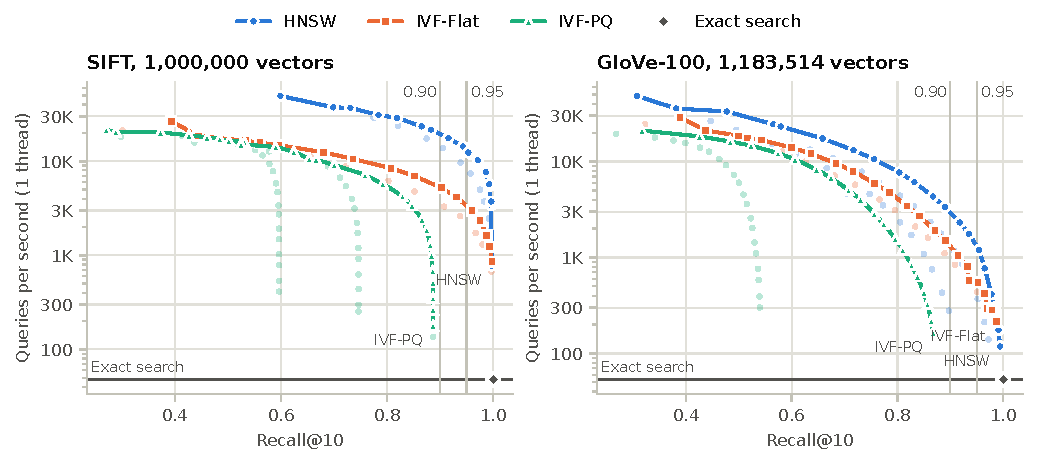
\includegraphics[width=\linewidth]{part2_recall_qps}
\caption{Recall@10 against single-thread QPS on a log scale. Each line is an index's best trade-off curve, the Pareto front over all its build and search settings, chosen on queries 0--4,999 and plotted on queries 5,000--9,999. Faint dots show every configuration, and grey shows exact search.\label{fig:part2}}
\end{figure}

\begin{table}[h]\centering
\tableinput{part2_qps_at_recall}\\[4pt]
\tableinput{part2_cost_at_095}
\caption{The top table gives the QPS of the fastest setting whose tune-half recall reaches 0.90 or 0.95, with its report-half recall. The bottom table gives the cost of the 0.95 setting. IVF-PQ never reaches 0.95, so the table shows its highest-recall setting, marked with *. Size is the serialised index, and the last column is the precomputed distance table that IVF-PQ also keeps in RAM.\label{tab:part2}}
\end{table}

% =====================================================================================================================
\section{Part 3: Scaling}
The benchmark ran again on the first 100K, 300K and 1M SIFT vectors and measured the cost of reaching recall 0.95 at each size
(Figure~\ref{fig:part3}, Table~\ref{tab:part3}). HNSW kept $M = 16$, and IVF-Flat used nlist = round($4\sqrt{N}$) (1,265, 2,191
and 4,000), so each list holds about $\sqrt{N}/4$ vectors. Exact search grew in proportion to $N$, as the hypothesis predicted. Its
latency slope on log-log axes is 1.05, and it computes exactly $N$ distances. IVF-Flat grew more slowly, with slope 0.65, but
faster than the predicted $\sqrt{N}$ (slope 0.5). The assumption behind that prediction did not hold. The number of lists needed
for 0.95 rose from 32 to 48, so the distance count grew with slope 0.62 instead of 0.5. HNSW grew slowest, with slope 0.42 (2.7$\times$ over the 10$\times$ range). That matches the predicted order but not the $\log N$ rate, which would give a slope of
only about 0.08 here. The efSearch needed rose from 32 to 64, because more vectors means more close candidates to compare. Each
distance also became slower (about 62\,ns at 100K and 81\,ns at 1M), probably because the larger graph fits the CPU cache less
well, though the benchmark did not measure cache misses. Overall the hypothesis held for exact search and for the order of the three methods,
but both indexes scaled worse than the idealised $\sqrt{N}$ and $\log N$ rates.

\begin{figure}[h]\centering
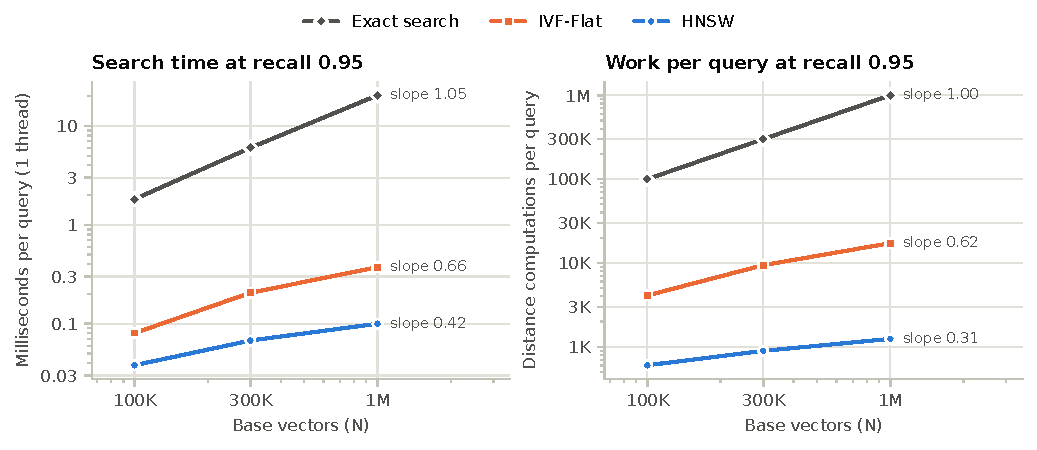
\includegraphics[width=\linewidth]{part3_scaling}
\caption{SIFT at 100K, 300K and 1M vectors. The left panel shows latency at each index's recall-0.95 setting, and the right panel shows distance computations per query at the same settings. Each label is the fitted log-log slope.\label{fig:part3}}
\end{figure}

\begin{table}[h]\centering
\tableinput{part3_growth}
\caption{Growth from 100K to 1M and the fit used for Q4. The slopes come from fits on log-log axes, for latency in ms and for distance computations. The fit interpolates latency at 150K and extrapolates it 10$\times$ beyond the data at 10M. Memory is the bytes per vector at 1M $\times$ N.\label{tab:part3}}
\end{table}

% =====================================================================================================================
\section{Part 4: Hard geometry}
The harder data comes from adding seeded Gaussian noise to the first 150,000 SIFT vectors and to all queries. Each coordinate gets
noise with standard deviation $\sigma \cdot s$, where $s$ = 32.75 is the mean per-coordinate standard deviation of the clean
vectors. Every level scales the same noise pattern (seed 42), so $\sigma$ is the only thing that changes. The levels are
$\sigma = 0$ as the unchanged control and 0.1, 0.3 and 1.0 as the noisy levels, 480,000 generated vectors in total. Each level gets its own ground truth and its own HNSW ($M = 16$) and IVF-Flat (nlist = 1024) builds. Figure~\ref{fig:part4} shows the
results. As intended, the relative contrast, the mean distance divided by the nearest-neighbour distance, fell from 2.42 to 1.52, so
a query's nearest neighbour became barely closer than a typical vector. Up to $\sigma = 0.3$ neither index changed much, but at
$\sigma = 1$ both lost recall. With the settings that reached 0.95 on the control, HNSW's recall fell from 0.976 to 0.728 and
IVF-Flat's from 0.968 to 0.806. Getting back to 0.95 needed efSearch 256 instead of 48 and nprobe 128 instead of 32. That made HNSW 5.8$\times$ slower and IVF-Flat 3.5$\times$ slower, so HNSW's lead shrank from 2.1$\times$ to 1.3$\times$ (2,929 vs 2,228 QPS). Exact search,
the control for cost, stayed at about 350 QPS, so the slowdowns come from the indexes and not from the data size.

This does not support the hypothesis that IVF-Flat would break most. HNSW lost more recall at a fixed setting and more speed to
recover. A likely mechanism, not tested here, is that HNSW moves greedily to whichever neighbour is closer. When all distances are
nearly equal, noise dominates those comparisons, so the search stalls in local minima and needs a wider beam. IVF-Flat chooses
lists by distance to centroids, which are averages of about 150 vectors each. Much of the noise cancels in these averages, so the nearest centroids still identify the lists that hold the true neighbours, and probing four times as many lists was enough. The experiment did not test
anisotropic or clustered noise, IVF-PQ, noise levels above 1, or other values of $N$, $M$ and nlist.

\begin{figure}[h]\centering
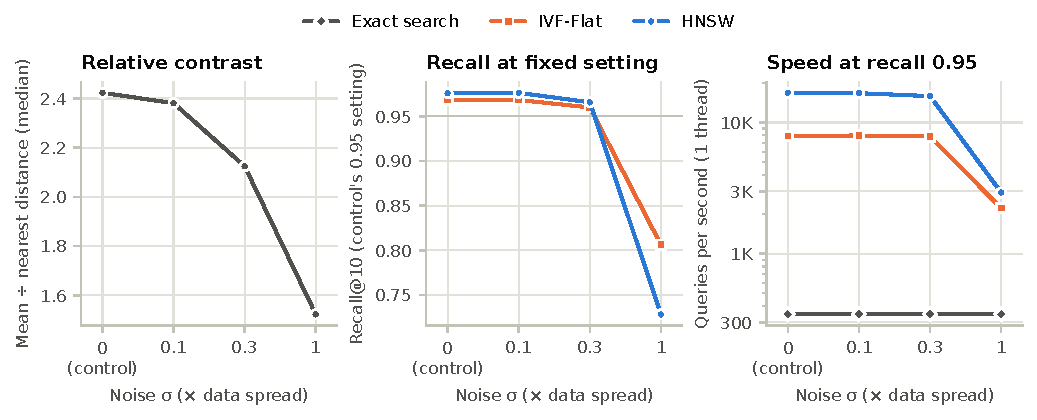
\includegraphics[width=\linewidth]{part4_noise}
\caption{Seeded Gaussian noise on 150K SIFT vectors. The left panel shows relative contrast. The middle panel shows recall when each index keeps the setting that reached 0.95 on the control. The right panel shows QPS at each noise level's own 0.95 setting, with exact search as the control for cost.\label{fig:part4}}
\end{figure}

% =====================================================================================================================
\section{Answers}
\paragraph{Q1. Fastest at recall 0.95.}
HNSW is the fastest at recall 0.95 on both datasets, with 10,951 QPS on SIFT and 1,198 on GloVe, 3.7$\times$ and 2.2$\times$ faster than IVF-Flat. The winner does not change, but its margin shrinks. Both indexes are slower on GloVe, HNSW by 9.1$\times$ and IVF-Flat by 5.4$\times$. HNSW needed $M = 32$ and efSearch 384 there instead of $M = 16$ and 64, and IVF-Flat needed nprobe 384
instead of 48. The distance counts explain both results. On SIFT, HNSW computes 13.7$\times$ fewer distances than IVF-Flat (1,245
vs 17,030 per query) but is only 3.7$\times$ faster, because each of its distances costs about 73\,ns against 20\,ns for IVF-Flat.
HNSW reads nodes from scattered places in memory, while IVF-Flat reads its lists sequentially, at the same speed per distance as
exact search. On GloVe both indexes need about 6--10$\times$ more distances for the same recall, probably because word vectors have
weaker neighbourhood structure, with many points almost equally far from a query.

\paragraph{Q2. Build time and memory, and what PQ saves and gives up.}
Building HNSW took 52.0\,s on SIFT ($M = 16$) and 107.4\,s on GloVe ($M = 32$). IVF-Flat took 43--48\,s, mostly for k-means with
4,096 centroids. IVF-PQ took 68.8\,s on SIFT because it also trains the PQ codebooks, and exact search only copies the vectors
(0.1\,s). In memory, exact search and IVF-Flat store the raw vectors (512 and 522 bytes per vector on SIFT), with IVF-Flat adding an
8-byte id. HNSW adds its graph links on top (656 bytes). IVF-PQ stores a 64-byte code instead of each vector, so its saved index is
only 74 bytes per vector, 7$\times$ smaller than IVF-Flat. The saving in RAM is smaller, because FAISS keeps a 268\,MB precomputed
distance table (nlist $\times$ $m$ $\times$ 256 floats) for fast search. IVF-PQ therefore uses 343\,MB against 522\,MB for IVF-Flat,
about 1.5$\times$ less. PQ gives up accuracy in return. It never reaches recall 0.90, and its best recall (0.887 on SIFT) needs
nprobe 768, where it is slower (179 QPS) than IVF-Flat at 0.95.

\paragraph{Q3. What Parts 3 and 4 imply about the headline numbers.}
The headline numbers of Part 2 hold for one dataset size and one kind of data. Part 3 shows that the settings that reach 0.95 at
1M vectors are not enough for larger collections, since efSearch and nprobe had to grow with $N$. It also shows that the cost grows
faster than the idealised $\sqrt{N}$ and $\log N$ rates, so a benchmark at one size understates the cost at a larger one. Part 4
shows that on data with lower contrast the same index needs several times more work (5.6$\times$ more distances for HNSW and
3.4$\times$ for IVF-Flat at $\sigma = 1$) or loses up to 0.25 recall at fixed settings. The gap between indexes can also change, and HNSW's lead over IVF-Flat shrank from 2.1$\times$ on clean data to 1.3$\times$ at $\sigma = 1$. SIFT is the easier of the two datasets,
and GloVe already shows the gap, so headline numbers on easy data can mislead about harder real data.

\paragraph{Q4. 150K or 10M vectors, 100 ms per query, 16 GB.}
For 150,000 vectors, ANN is not worth using. Based on the exact-search timings, one query takes about 2.86\,ms, 35$\times$ inside
the 100\,ms budget, with perfect recall, no build time and 0.08\,GB of memory. An index would help only if the application needed
many queries per second. For 10 million vectors, exact search would take about 236\,ms per query, over the budget, so the
recommendation is HNSW. On SIFT-like data, $M = 16$ extrapolates to about 0.28\,ms per query and 6.6\,GB, which fits in 16\,GB.
Harder data like GloVe needs $M = 32$ (about 6.7\,GB). efSearch needs re-tuning on held-out queries at the new size, because the
value needed for 0.95 grew with $N$ (32, 48, 64). IVF-Flat would also fit (5.2\,GB) and meet the budget (about 1.7\,ms), but it is
slower. PQ is not needed at this size and would cap recall below 0.9 without re-ranking. These 10M numbers extrapolate the fit
10$\times$ beyond the largest size measured, and the benchmark did not measure build time at that size.

\paragraph{Q5. Two ways this benchmark could mislead.}
First, all speeds here are for one query at a time on one thread. That is the latency a single user sees, but not how a server
handles load. Part 1 shows how much this can change the numbers, since batching made exact search 3.3$\times$ faster on one thread and 16.2$\times$ faster on 12. The benchmark tested this only for exact search. It never timed the ANN indexes in batches or with several threads, so their ranking under a throughput-oriented load is untested. Second, measuring index size as the size of the saved index
understates the memory IVF-PQ needs, because FAISS rebuilds a 268\,MB precomputed distance table when it loads the index. The benchmark tests this one. It measures the table and reports it next to the size, which shrinks PQ's memory saving from 7$\times$ to
about 1.5$\times$.

\end{document}
